\documentclass[12pt, a4paper]{article}
\makeatletter
\def\@fnsymbol#1{\ensuremath{\ifcase#1\or 1\or 2\or
		3\or \mathparagraph\or \|\or **\or \dagger\dagger
		\or \ddagger\ddagger \else\@ctrerr\fi}}
\makeatother
\usepackage[
backend=biber
]{biblatex}
\usepackage{icomma}
\usepackage{fontspec}
\setmainfont[BoldFont={Calibri, Bold},ItalicFont={Calibri, Italic}]{Calibri}
\renewcommand{\baselinestretch}{1} 
\usepackage{geometry}
\geometry{
	a4paper,
	right =20mm,
	left=20mm,
	bottom = 15mm,
	top=20mm
}
\usepackage[italian]{babel}
\usepackage{hyperref}
\usepackage{float}
\usepackage{subcaption}
\usepackage{graphicx}
\graphicspath{ {.} }
\addbibresource{bib.bib}
\usepackage{tikz}
\usetikzlibrary{shapes,arrows}
\usepackage{pgfplots}
\pgfplotsset{width=8cm,compat=1.9}
\usetikzlibrary{pgfplots.dateplot}
\usepackage{pgfplotstable}
\usepackage{filecontents}
\usepackage[utf8]{inputenc} %codification of the document
\title{Stazione meteorologica Open Source\\\Large{Monitoraggio ambientale decentralizzato e scolastico}}
\author{Mattia Mascarello\thanks{Design del software, m2.mascarello@liceococito.it}\and Lorenzo Dellapiana\thanks{Design elettronico, l.dellapiana@liceococito.it}\and Luca Savio Biello\thanks{Analista di progetto, ls.biello@liceococito.it}}
%Here begins the body of the document
\date{\parbox{\linewidth}{\centering%
		\today\endgraf\bigskip
		Liceo Scientifico Statale ``Leonardo Cocito''}}
\begin{document}
	\maketitle
	
	\begin{abstract}
		Negli ultimi tempi, l'opinione pubblica è diventata più consapevole delle questioni legate all'ambiente, in particolare il riscaldamento globale causato da $CO_2$ e altri gas serra emessi nell'atmosfera dall'attività umana e  degli altri effetti negativi causati dall'inquinamento che colpiscono la salute umana e gli ecosistemi.
		Il nostro team ha ideato un progetto che prevede la costruzione di una rete di stazioni meteorologiche costruite con componenti relativamente economici, che può essere svolta come attività extracurriculare o curriculare (cioè attinente al programma di informatica) nelle scuole coinvolte nel progetto.
		Viene fornito un kit software open source espandibile e adattabile per il completamento dell'attività, ma gli studenti possono fornire le proprie soluzioni a condizione che i risultati prodotti rispettino lo standard per lo scambio di dati.
		I dati raccolti saranno quindi visualizzabili pubblicamente sul sito web della scuola attraverso una pagina web, pubblicati come repository di dati aperti, pubblicamente accessibili e interrogabili e aggiunti all'elenco delle fonti di dati che il progetto mantiene.
		La raccolta di dati preziosi (che include ma non si limita a qualità dell'aria, umidità, temperatura e pressione) ha il valore aggiunto di insegnare agli studenti elementi di informatica (in particolare, interfacciamento con hardware, archiviazione dati e comunicazioni di rete), statistica e meteorologia.
		Le misurazioni raccolte potrebbero essere utilizzate anche per fornire uno strumento decisionale alle autorità locali o per integrare i dati del governo laddove le infrastrutture per la qualità dell'aria siano assenti o scarse.
		Se l'iniziativa dovesse essere ampiamente adottata, sarebbe possibile creare mappe e modelli su larga scala per previsioni, misurazioni e monitoraggio della qualità dell'aria.
	\end{abstract}
	
	\clearpage
	\tableofcontents
	\clearpage
	\renewcommand{\abstractname}{Riconoscimenti}
	\begin{center}
		\begin{abstract}
			\vspace{10mm}
			Ringraziamo tutti coloro che hanno sostenuto e aiutato questo progetto\\
			\vspace{10mm}
			\textbf{Professori}\\
			prof. Claudia Abrigo, Scienze\\
			prof. Loredana Ercolini, Scienze\\
			prof. Daniela Genta, Matematica e Fisica\\
			prof. Andrea Piccione, Matematica e Fisica\\
			prof. Cinzia Bori, Inglese\\
			\vspace{10mm}
			\textbf{Studenti}\\
			Leonardo Agnoletto, 4G\\
			Arsildo Gjoka, 4G\\
			Gaia Gnecchi, 5D\\
			Sofia Pressenda, 4G,\\
			Elia Taliano, 4G\\
			\vspace{10mm}
			\textbf{Referente}\\
			prof. Marina Orazietti, Scienze\\
		\end{abstract}
	\end{center}
	
	\clearpage
	\section{Preambolo}
	Il team si è concentrato sulla costruzione di un prototipo di stazione meteorologica da utilizzare in modo scalabile e gestibile attraverso una potenziale rete di centinaia di nodi.
	Gli obiettivi di progettazione erano: costi ridotti, facilità di creazione e autonomia di funzionamento dell'apparato.
	
	\section{Hardware}
	La stazione meteorologica è composta da tre parti: un microprocessore ARDUINO MEGA 2560, un computer RASPBERRY 3B+ e due sensori di qualità dell'aria.
	\subsection{Controllori principali}
	
	\begin{itemize}
		\item \emph{ARDUINO MEGA 2560}: microcontrollore basato sull'architettura ATMega2560 (clock a 16 Mhz), che fornisce 54 pin per I/O digitale e 16 pin per I/O analogico.\\ 
		\item \emph{RASPBERRY PI 3B+}: PC basato su ARM dotato di senseHat (un ``cappello'' con matrice di led, sensori di umidità, temperatura e pressione), 4 porte usb, funzionalità di rete wireless e cablata.
	\end{itemize}
	
	\subsection{Sensori di qualità dell'aria}
	La scheda \emph{Arduino} invia i dati tramite una connessione USB seriale al Raspberry Pi ed è collegata a due sensori:\\
	\emph{FC22} (\emph{fig. \ref{fig:fc22}}): raccoglie dati su fumo e vapori infiammabili e ne determina la concentrazione nell'aria ($\frac{\mu g}{m^3}$).\\
	\emph{SDS011} (\emph{fig. \ref{fig:sds011}}): determina la concentrazione di particelle sospese nell'aria, ovvero PM10 (con un diametro inferiore a $10\mu m$) e PM2.5 (con un diametro inferiore a $2,5 \mu m$).\\
	Il \emph{SenseHat} invece si interfaccia direttamente con il Raspberry Pi, e quindi i dati di temperatura, umidità e pressione sono registrati direttamente con la sua API Python.\\
	La presenza delle due unità ha una utilità didattica rilevante, siccome presuppone l'approcciarsi a due linguaggi di programmazione diversi (\texttt{C} e \texttt{Python}), paradigmi e interfacce hardware diverse, pur conservando allo stesso tempo una utilità materiale (il sensore di qualità dell'aria opera ad una differenza di potenziale incompatibile con il Raspberry).
	\subsection{Specifiche dei sensori}
	\begin{table}[H]
	\caption{Precisione dei dati}
	\begin{tabular}{|l|l|l|}
	\hline
	Sensore & Intervallo di funzionamento & Precisione\\
	\hline
	\hline
	Barometro & $[260,1260]hPa$ & $\pm0,1hPa$\\
	\hline
	Termometro & $[-40,+120]°C$ & $\pm 0,5 °C$\\
	\hline
	Igrometro & $[20,90]\%$ & $\pm 4,5\%$\\
	\hline
	Rilevatore PM10 e PM2,5 \emph{(SDS011)}& $[0,999.9]\frac{\mu g}{m^3}$ & $\pm 10\frac{\mu g}{m^3}$\\
	\hline
	Rilevatore fumo e vapori infiammabili \emph{(FC22)} &$[10,1000]\frac{\mu g}{m^3}$ & $\pm 10\frac{\mu g}{m^3}$\\
	\hline
	\end{tabular}
	\end{table}
	\clearpage
	\begin{figure}[H]
		\centering
		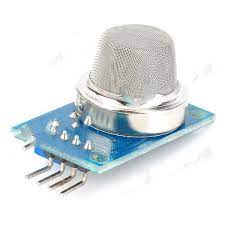
\includegraphics[]{FC22.png}\\
		\caption{\emph{FC22}}
		\label{fig:fc22}
	\end{figure}
	\begin{figure}[H]
		\centering
		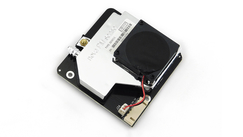
\includegraphics[]{sds011.jpg}\\
		\caption{\emph{SDS011}}
		\label{fig:sds011}
	\end{figure}
	\begin{figure}[H]
		\centering
		%\includegraphics[width=1.0\textwidth]{Image.eps}
		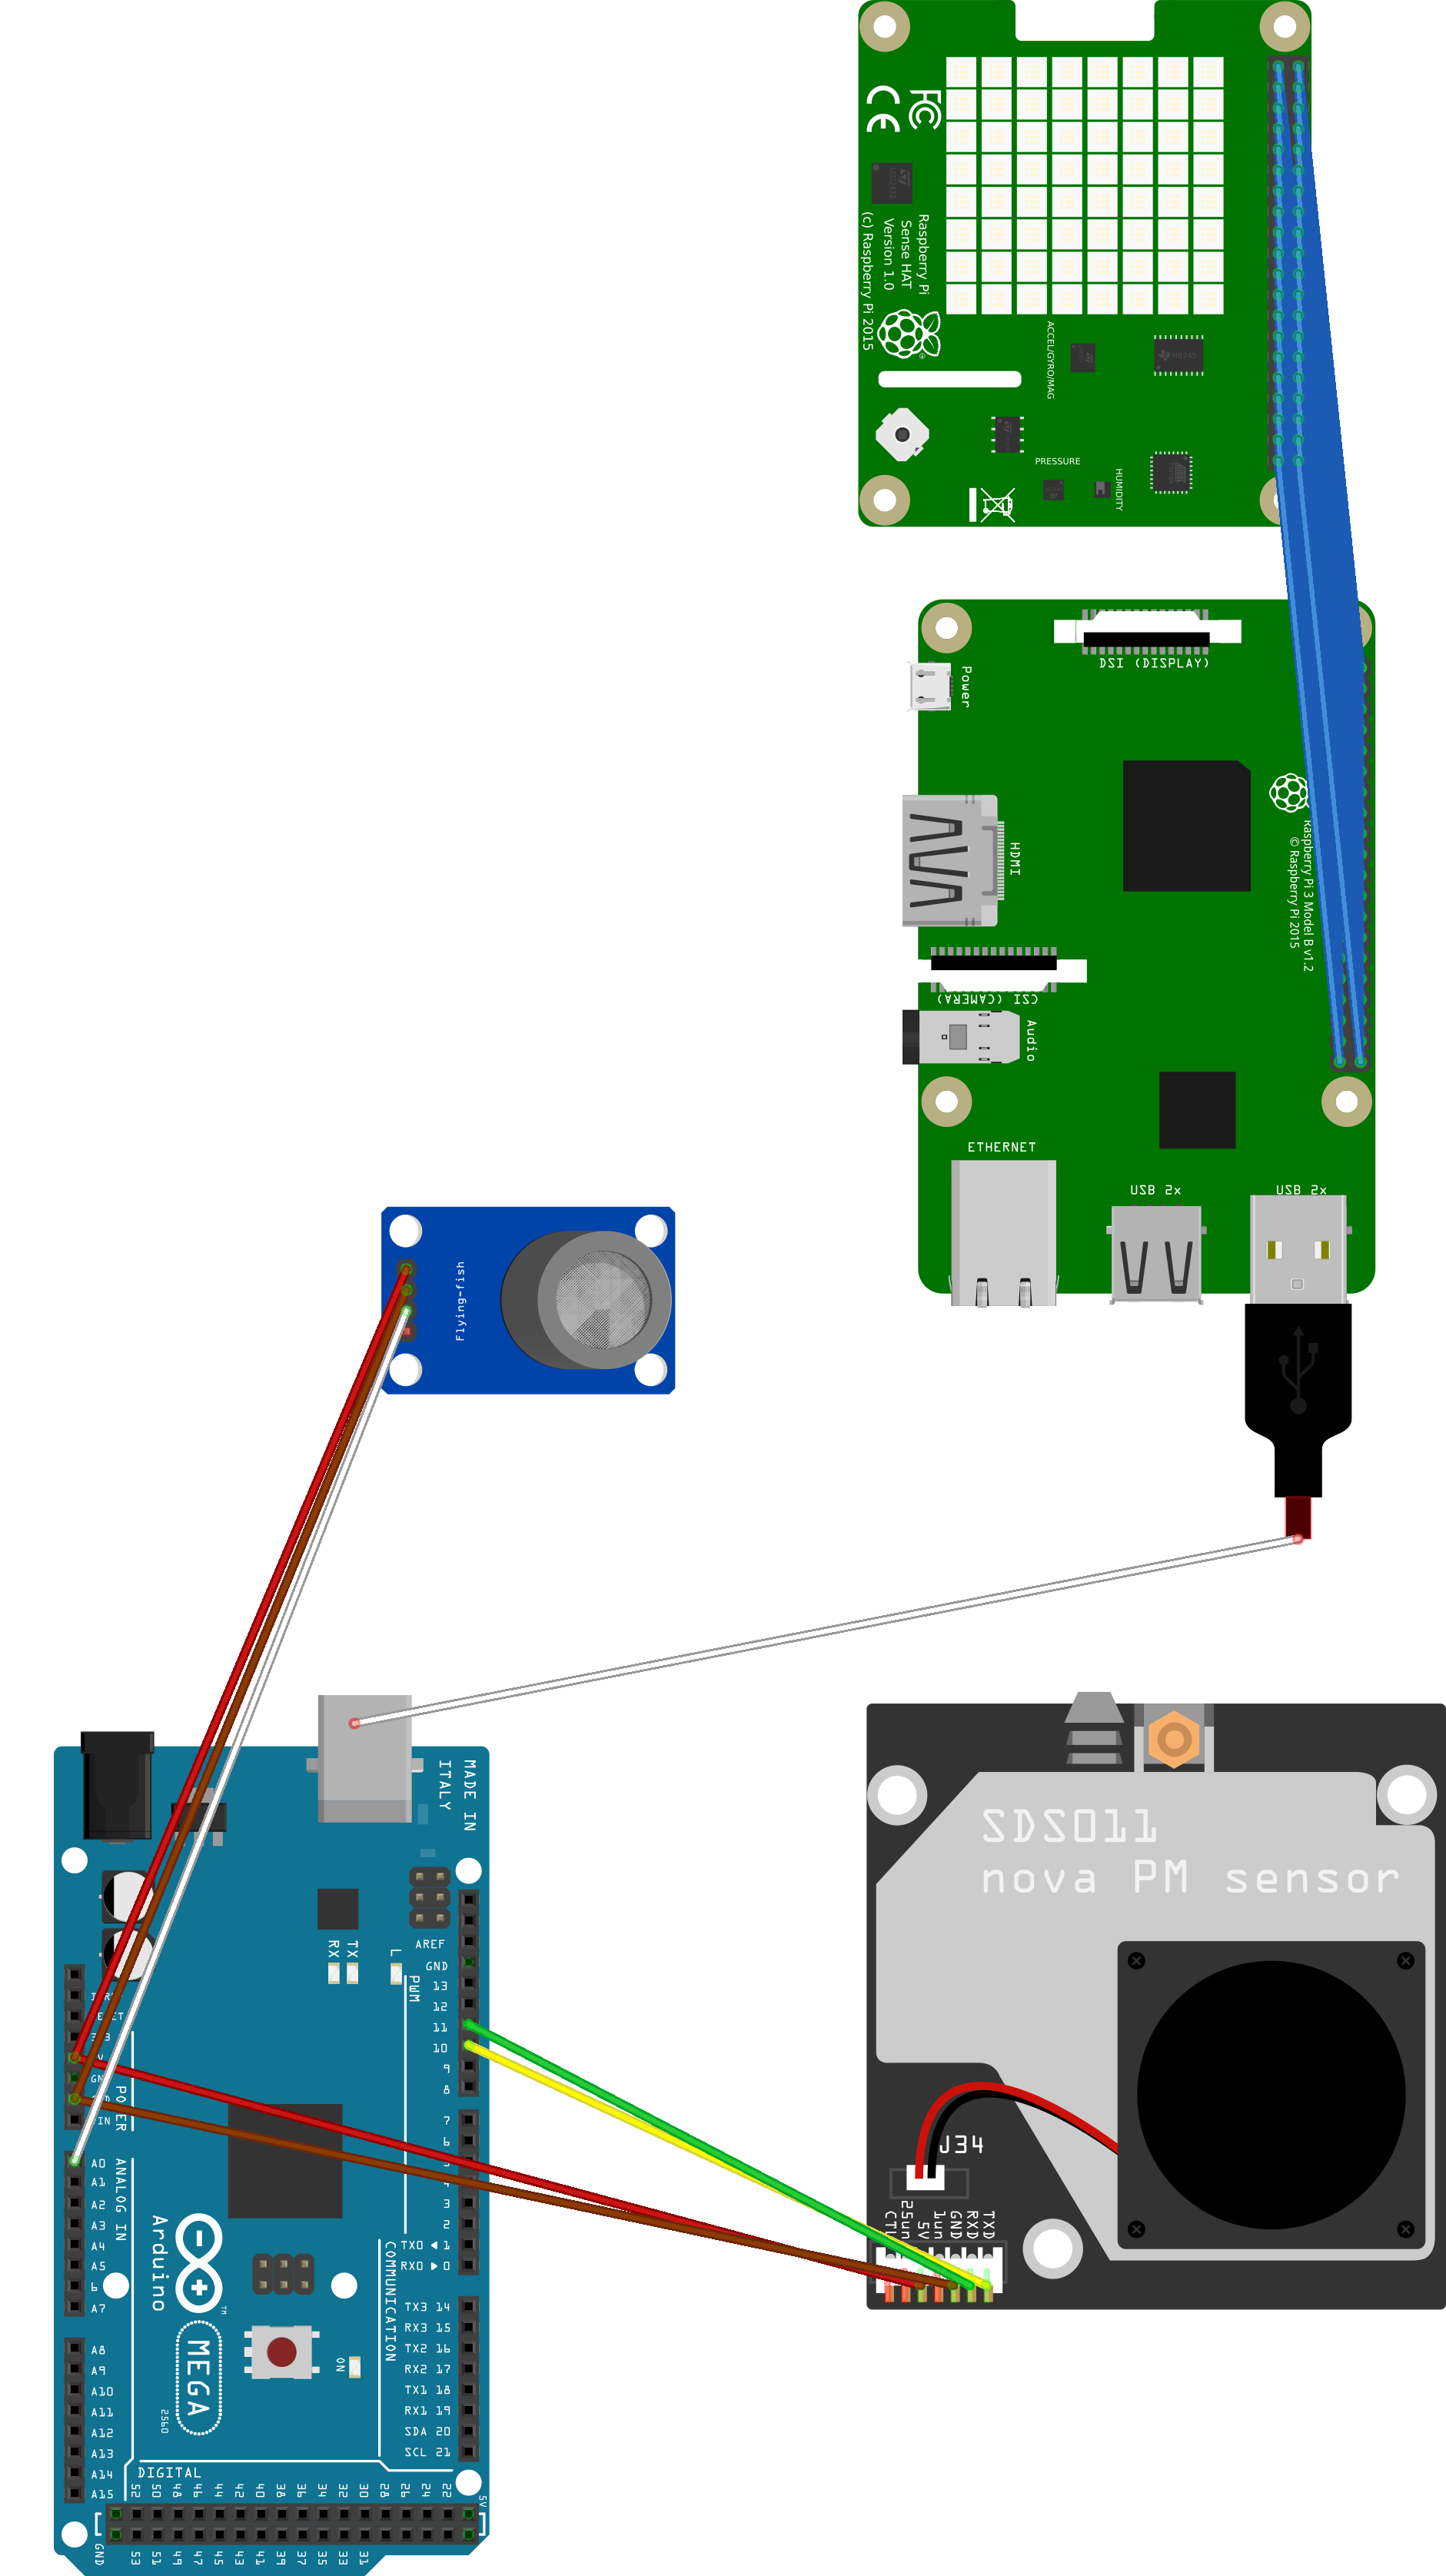
\includegraphics[height=0.95\textheight]{board.png}
		\caption{Ricostruzione della disposizione delle componenti}
		\label{fig:board}
	\end{figure}
	\clearpage
	\begin{figure}[H]
		\centering
		%\includegraphics[width=1.0\textwidth]{Image.eps}
		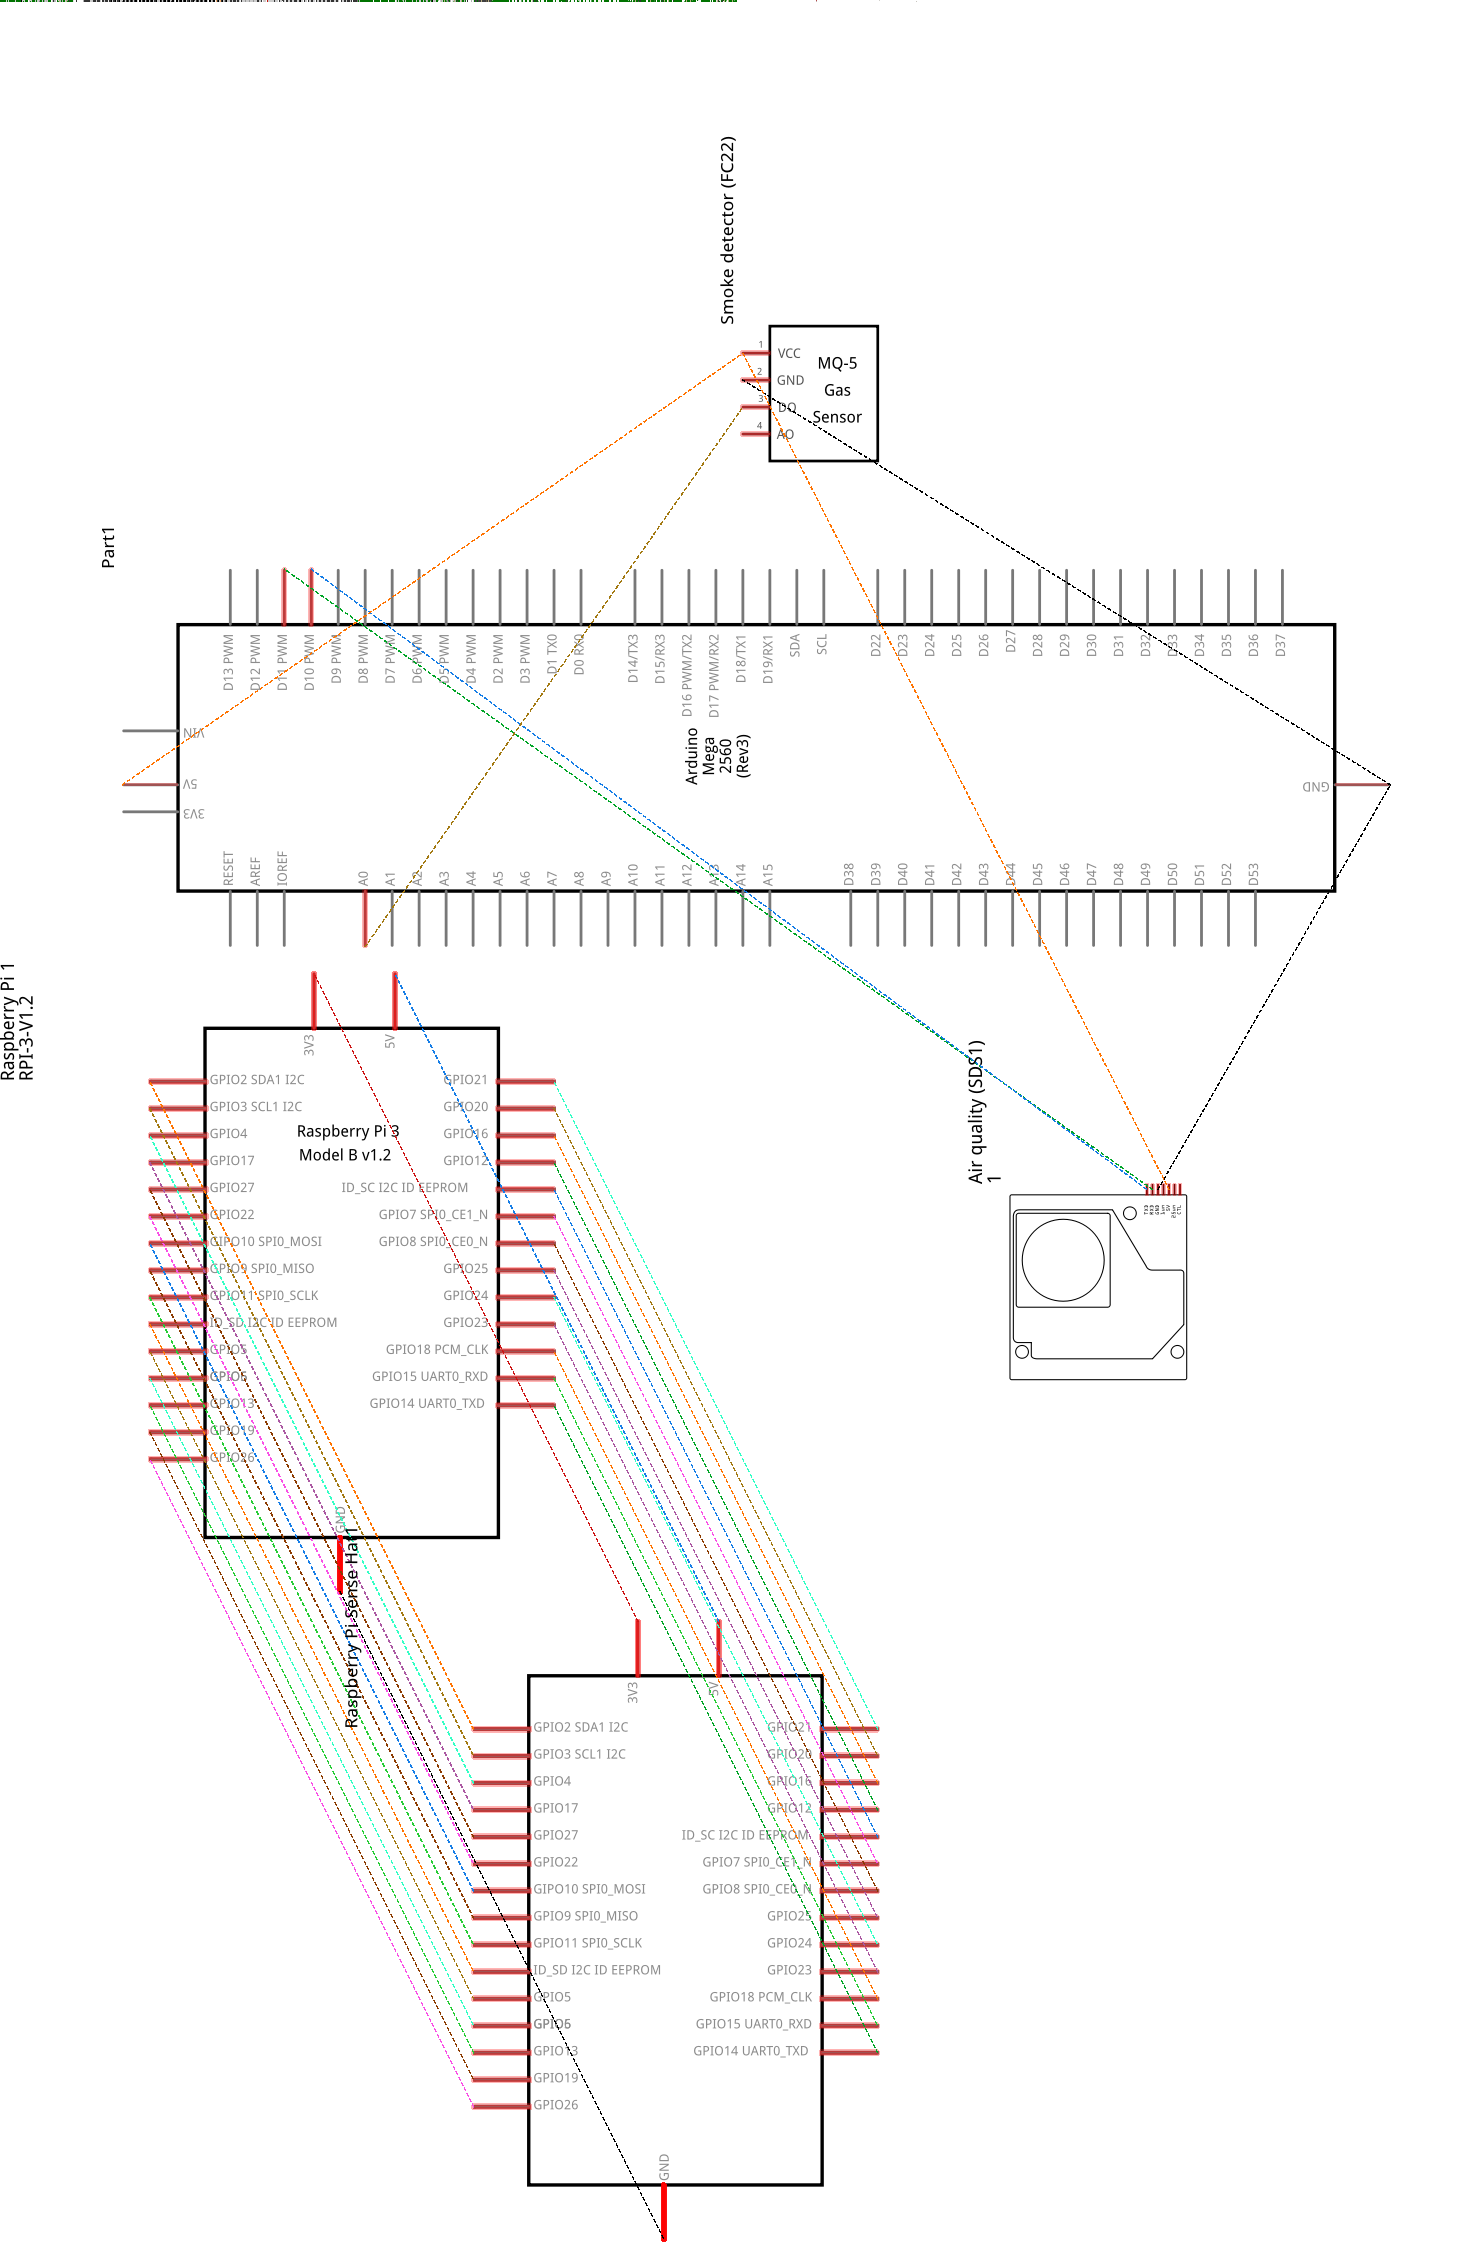
\includegraphics[height=0.95\textheight]{schema.png}
		\caption{Diagramma delle componenti}
		\label{fig:schema}
	\end{figure}
	\clearpage
	
	\subsection{Presentazione dei dati}
	\subsubsection{Display}
	Un'unità separata, dotata di un display da $7''$ (controllato da un \emph{Raspberry Pi 3B+}), scarica e mostra i dati recenti e storici ai passanti e può quindi essere posizionata in un luogo dove è più visibile, come un corridoio di una scuola.\\
	
	Sono disponibili due cruscotti: un display analogico con quadranti e un display digitale minimalista ``neon'' per una facile lettura.
	\subsubsection{Sito web}
	
	Un server web ottiene i dati dall'archivio \emph{git} e li visualizza in grafici e tabelle relativi a diversi periodi di tempo.
	
	\subsubsection{Repository}
	
	Una \emph{repository} \emph{git} contiene le misurazioni che vengono salvate in file in formato \emph{csv}.
	La struttura del percorso del file è \texttt{aaaa/mm/gg/tipo.csv}.
	
	\begin{table}[H]
		\caption{Formato dati}
		\begin{tabular}{|l|l|l|l|l|}
			
			\hline		
			Tipo di dato   & Formato                                                                                                                        & Unità di misura & \multicolumn{1}{l|}{Tipo di file}     & Precisione    \\
			\hline		
			\hline		
			Datetime        & \begin{tabular}[c]{@{}l@{}}aaaa-mm-gg hhh:mm:ss\\ \textbf{Attenzione}: L'ora è espressa in \\ ``CET'' (+1),  l'ora \\locale italiana\end{tabular} & - &- &-                                                 \\ 
			\hline		
			Temperature & decimale                                                                                                                       & $°C$                & \multicolumn{1}{l|}{\texttt{temperature.csv}} &  $\pm 0,5°C$ \\
			\hline		
			Umidità    & decimale                                                                                                                       & $\%$                & \multicolumn{1}{l|}{\texttt{humidity.csv}} & $\pm 4,5\%$   \\ 
			\hline		
			Pressione    & decimale                                                                                                                       & $hPa$                 & \multicolumn{1}{l|}{\texttt{pressure.csv}}  & $\pm 0,1hPa$   \\ 
			\hline		
			Fumo       & decimale                                                                                                                       & $\frac{\mu g}{m^3}$               & \multicolumn{1}{l|}{\texttt{smoke.csv}}    &  $\pm 0,3 \mu\frac{g}{m^3}$  \\ 
			\hline		
			PM10        & decimale                                                                                                                       & $\frac{\mu g}{m^3}$               & \multicolumn{1}{l|}{\texttt{pm10.csv}}     &  $\pm 0,3 \mu\frac{g}{m^3}$     \\ 
			\hline		
			PM2.5       & decimale                                                                                                                       & $\frac{\mu g}{m^3}$               & \multicolumn{1}{l|}{\texttt{pm25.csv}}      &  $\pm 1 \mu\frac{g}{m^3}$   \\
			\hline		
		\end{tabular}
	\end{table}
	La \emph{repository} contiene anche un report testuale sullo stato di operatività della stazione (\texttt{report.txt}), insieme ad un file contente gli ultimi dati in formato \texttt{json} (\texttt{latest.json}).
	\clearpage
	\begin{figure}[!h]
		\centering
		%\includegraphics[width=1.0\textwidth]{Image.eps}
		
\includegraphics[width=0.95\textwidth]{dash.png}
		\caption{Cruscotto}
		\label{fig:dash}
	\end{figure}
	
	\begin{figure}[!h]
		\centering
		%\includegraphics[width=1.0\textwidth]{Image.eps}
		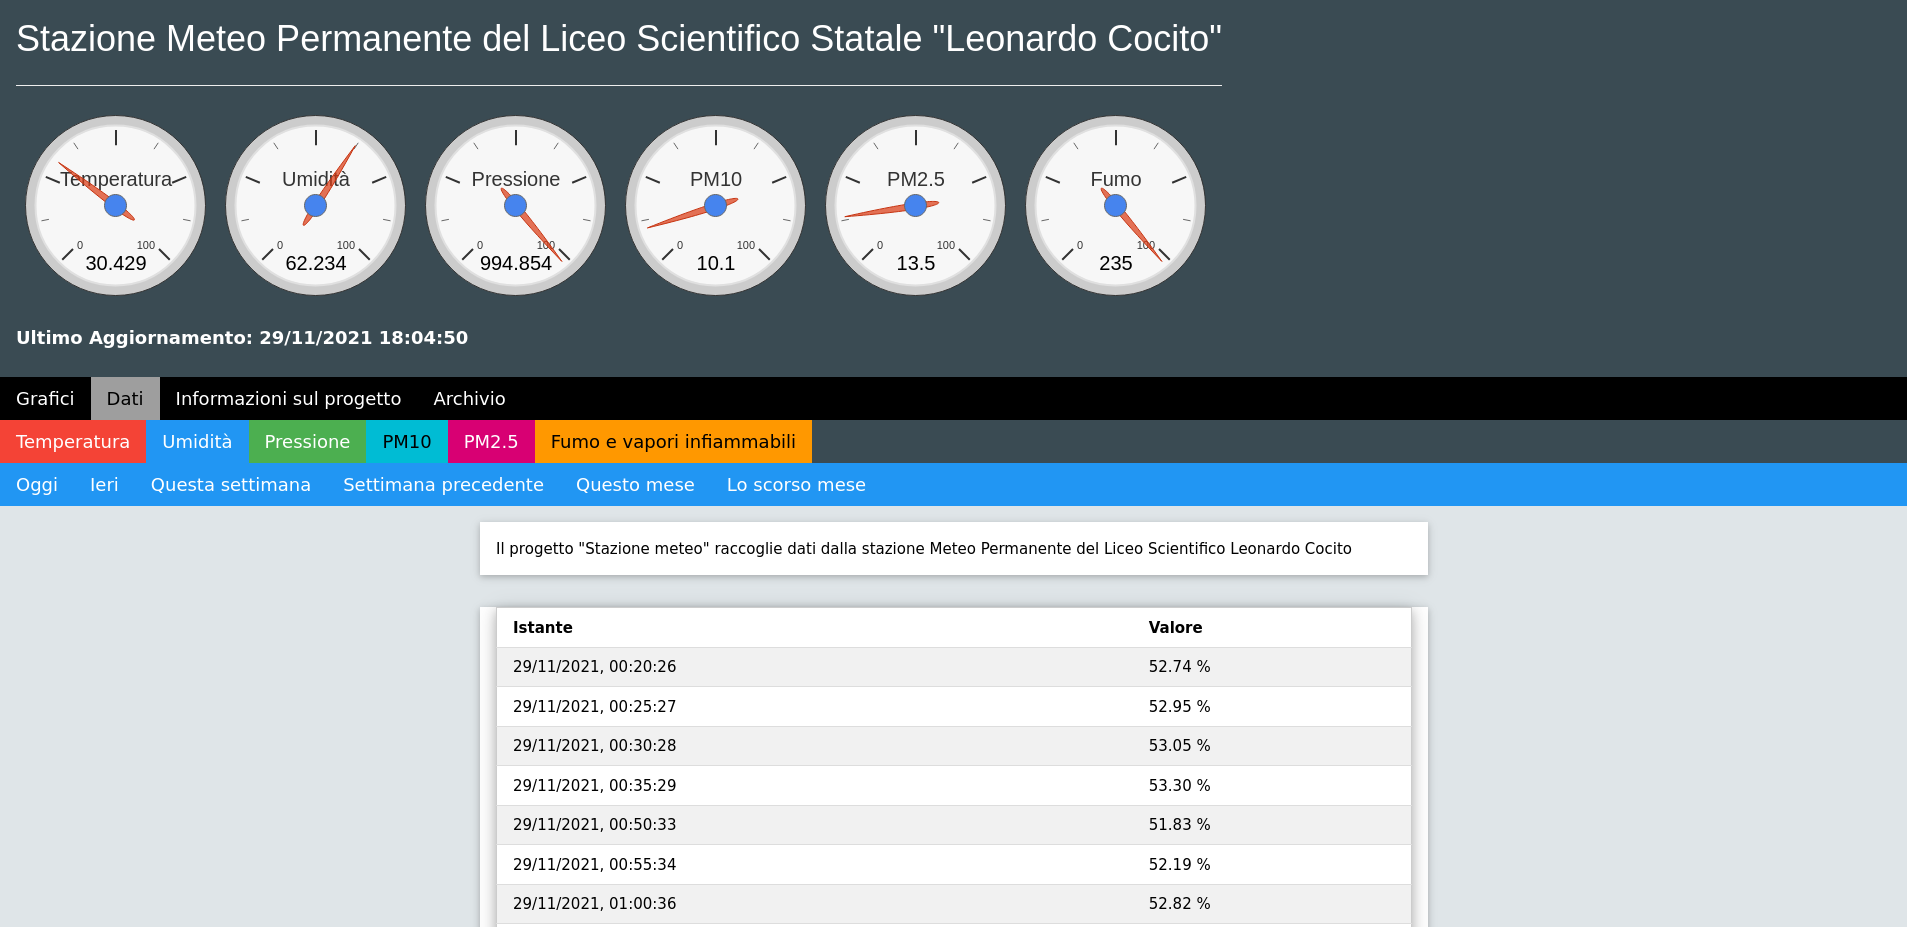
\includegraphics[width=0.95\textwidth]{web.png}
		\caption{Sito web}
		\label{fig:web}
	\end{figure}
	\clearpage
	
	\section{Software}
	Il codice sorgente è memorizzato in una repository git all'indirizzo  \url{http://www.github.com/MatMasIt/weatherStation}.\\
	Il kit contiene tutti gli strumenti necessari per l'acquisizione, il trasferimento, l'archiviazione e la pubblicazione dei dati ed è stato sviluppato con l'ausilio di diversi linguaggi di programmazione per ottimizzare ogni attività.
	\section{Open data}
	La disponibilità di dati in formato aperto e standard consente di effettuare indagini comparative, rielaborazioni e da nuovo impulso alla realizzazione di stazioni che seguano lo stesso standard e che quindi possono facilmente unirsi alla rete e contribuire con i loro dati per rendere il processo di raccolta ancora più capillare ed efficace.
	
	\section{Rilevanza delle misurazioni}
	Il PM10 è stato ampiamente associato a problemi di salute \cite{pm101996}, aumento del tasso di cancro \cite{pm10} e, più recentemente, alla diffusione di COVID-19 \cite{pmcovid}.\\
	Inoltre, una raccolta accurata e geograficamente distribuita di questo tipo di dati deve ancora essere raggiunta, e il progetto che fornirebbe un grande set di dati meteorologici che potrebbe essere utilizzato per migliorare i modelli di previsione meteorologica esistenti e crearne di nuovi, pur essendo sempre didatticamente rilevante.\\

	I dati raccolti nel mese di dicembre sono stati confrontati con lo storico di una vicina stazione meteorologica dell' Agenzia Regionale per la Protezione Ambientale del Piemonte, e vengono qui mostrati per evidenziarne l'accuratezza e l'utilità.\\
	La stazione Open Source registra con maggiore precisione decimale e frequenza i cambiamenti delle variabili in questione, che ricadono negli intervalli indicativi del mese, tenendo conto della differenza di altitudine delle due stazioni prese in considerazione.
	\begin{figure}
		\begin{subfigure}{\linewidth}
				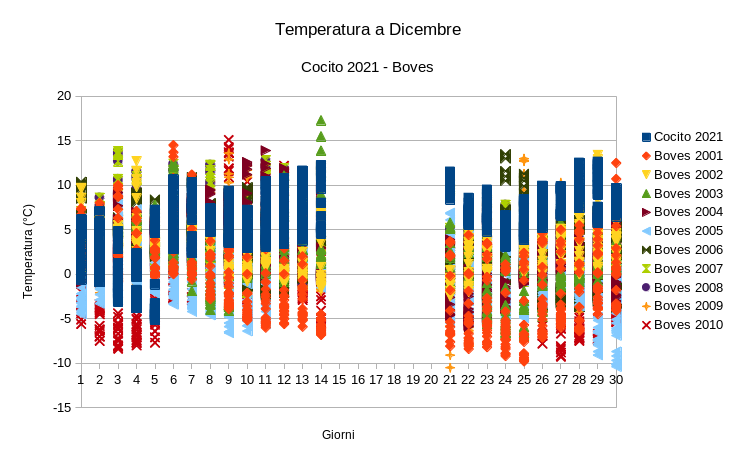
\includegraphics[height=150pt]{graficiBoves/temperatura.png}
				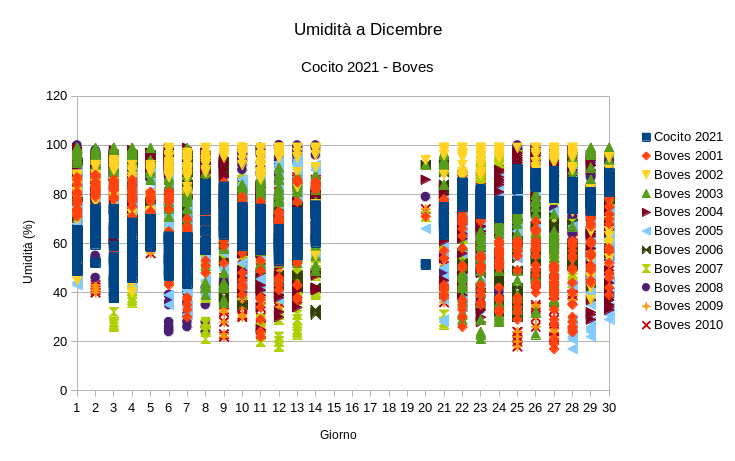
\includegraphics[height=150pt]{graficiBoves/umidita.png}
				\caption{}
			   \end{subfigure}\par\medskip
		      \begin{subfigure}{\linewidth}
		      	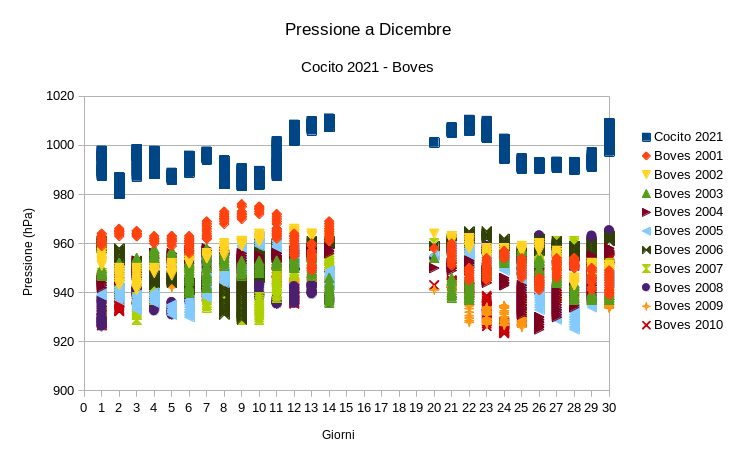
\includegraphics[height=300pt]{graficiBoves/pressione.png}
					\caption{}
				\end{subfigure} 
	\caption{Rilevazioni confrontate con i dati storici di una vicina stazione meteorologica dell' Agenzia Regionale per la Protezione Ambientale del Piemonte}
      \end{figure}
	\vfill
	\clearpage
	\begin{table}[H]
		\caption{Dati rilevati a dicembre 2021}
		\begin{tabular}{|l|l|@{}c@{}|}
			\hline
			Variabile Statistica & Calcolo & Valore\\
			\hline\hline
			Dimensione del campione & $N$ & \begin{tabular}{c|p{2cm}} Temperatura & $5005$ \\ \hline Umidità & $5005$ \\ \hline Pressione & $5002$ \\ \hline PM10 & $4998$\\ \hline PM2,5& $4998$\\ \hline Fumo e vapori infiammabili& $4998$ \end{tabular} \\
			\hline
			Massimo & $max$ & \begin{tabular}{c|p{2cm}} Temperatura & $21,13°C$ \\ \hline Umidità & $90,85 \%$ \\ \hline Pressione & $ 	1'011,03 hPa$ \\ \hline PM10 & $143,70\frac{\mu g}{m^3}$\\ \hline PM2,5& $156,10\frac{\mu g}{m^3}$\\ \hline Fumo e vapori infiammabili& $420,00\frac{\mu g}{m^3}$ \end{tabular} \\
			\hline
			Minimo & $min$ & \begin{tabular}{c|p{2cm}} Temperatura & $-7,34°C$ \\ \hline Umidità & $34,97 \%$ \\ \hline Pressione & $980,04 hPa$ \\ \hline PM10 & $4\frac{\mu g}{m^3}$\\ \hline PM2,5& $5,40\frac{\mu g}{m^3}$\\ \hline Fumo e vapori infiammabili& $130,00\frac{\mu g}{m^3}$ \end{tabular} \\
			\hline
			Media aritmetica & $\mu=\frac{\sum_{i=1}^{N}x_i}{N}$ & \begin{tabular}{c|p{2cm}} Temperatura & $4,96°C$ \\ \hline Umidità & $68,5 \%$ \\ \hline Pressione & $995,3 hPa$ \\ \hline PM10 & $32,99 \frac{\mu g}{m^3}$\\ \hline PM2,5& $41,92 \frac{\mu g}{m^3}$\\ \hline Fumo e vapori infiammabili& $178,14 \frac{\mu g}{m^3}$ \end{tabular} \\
			\hline
			Deviazione Standard & 	$\sigma _{X}={\sqrt {\frac {\sum \limits _{i=1}^{N}(x_{i}-{\bar {x}})^{2}}{N-1}}}
			$ & \begin{tabular}{c|p{2cm}} Temperatura & $3,53°C$ \\ \hline Umidità & $10,48 \%$ \\ \hline Pressione & $8,25 hPa$ \\ \hline PM10 & $24,59 \frac{\mu g}{m^3}$\\ \hline PM2,5& $27,01 \frac{\mu g}{m^3}$\\ \hline Fumo e vapori infiammabili& $17,81 \frac{\mu g}{m^3}$ \end{tabular}  \\
			\hline
			Coefficiente di variazione & 	$ \sigma ^{*}={\frac {\sigma }{|\mu |}}$ & \begin{tabular}{c|p{2cm}} Temperatura & $0,71$ \\ \hline Umidità & $0,15$ \\ \hline Pressione & $8,28\cdot10^{-3}$ \\ \hline PM10 & $0,74$\\ \hline PM2,5& $0,64$\\ \hline Fumo e vapori infiammabili& $0,1$ \end{tabular} \\
			\hline
			Moda (intera)& 	$Mo$ & \begin{tabular}{c|p{2cm}} Temperatura & $6 °C$ \\ \hline Umidità & $74 \%$ \\ \hline Pressione & $995 hPa$ \\ \hline PM10 & $22\frac{\mu g}{m^3}$\\ \hline PM2,5&  $45\frac{\mu g}{m^3}$\\ \hline Fumo e vapori infiammabili&  $181\frac{\mu g}{m^3}$\end{tabular} \\
			\hline
		\end{tabular}
		\end{table}



	\section{Conclusioni}
	In conclusione, il team ha posto le basi e le istruzioni per la facile costruzione di stazioni di monitoraggio del meteo e della qualità dell'aria, in un modo didatticamente integrato che potrebbe essere perseguito da molte scuole e produrre un grande valore sia in termini didattici che di risultato, date le molteplici applicazioni che queste stazioni possono avere.
	\clearpage
	\printbibliography
\end{document}